\documentclass{beamer}
\usepackage{beamerthemesplit}
\usepackage{wrapfig}
\usetheme{SPbGU}
\usepackage{pdfpages}
\usepackage{amsmath}
\usepackage{cmap} 
\usepackage[T2A]{fontenc} 
\usepackage[utf8]{inputenc}
\usepackage[english,russian]{babel}
\usepackage{indentfirst}
\usepackage{amsmath}
\usepackage{tikz}
\usepackage{multirow}
\usepackage[noend]{algpseudocode}
\usepackage{algorithm}
\usepackage{algorithmicx}
\usetikzlibrary{shapes,arrows}
\usepackage{fancyvrb}

\usepackage{graphicx}
\usepackage[utf8]{inputenc}  
\usepackage{amsmath}
\usepackage{amssymb}
\usepackage{amsthm}
\usepackage{latexsym}
\usepackage{float}
\usepackage{tabularx}
\usepackage{booktabs}

\allowdisplaybreaks

\newtheorem{rutheorem}{Теорема}
\newtheorem{ruproof}{Доказательство}
\newtheorem{rudefinition}{Определение}
\newtheorem{rulemma}{Лемма}

\beamertemplatenavigationsymbolsempty

\title[]{Восходящий анализ. RNGLR}
\subtitle[]{}
% То, что в квадратных скобках, отображается в левом нижнем углу. 
\institute[]{
Санкт-Петербургский государственный университет \\
Математико-механический факультет }

% То, что в квадратных скобках, отображается в левом нижнем углу.
\author[Екатерина Вербицкая]{Екатерина Вербицкая}

\date{1 декабря 2015г.}

\definecolor{orange}{RGB}{179,36,31}

\begin{document}
{
\begin{frame}[fragile]
  \titlepage
\end{frame}
}

\begin{frame}[fragile]
  \transwipe[direction=90]
  \frametitle{GSS}
\begin{center}
  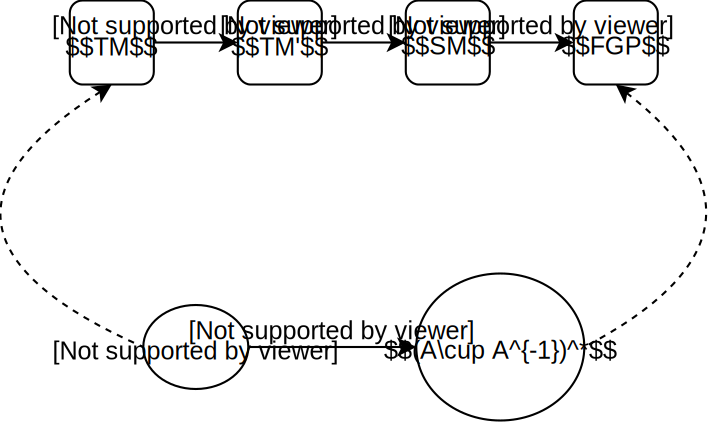
\includegraphics[width=1.0\textwidth]{pics/1}
\end{center}                                      
\end{frame}

\begin{frame}[fragile]
  \transwipe[direction=90]
  \frametitle{GSS}
\begin{center}
  \includegraphics[width=1.0\textwidth]{pics/2}
\end{center}                                      
\end{frame}

\begin{frame}[fragile]
  \transwipe[direction=90]
  \frametitle{Грамматика $\Gamma_1$}
\begin{center}
  \includegraphics[width=1.0\textwidth]{pics/3}
\end{center}                                      
\end{frame}

\begin{frame}[fragile]
  \transwipe[direction=90]
  \frametitle{Грамматика $\Gamma_2$}
\begin{center}
  \includegraphics[width=1.0\textwidth]{pics/4}
\end{center}                                      
\end{frame}

\begin{frame}[fragile]
  \transwipe[direction=90]
  \frametitle{Таблица для $\Gamma_2$}
\begin{center}
  \includegraphics[width=1.0\textwidth]{pics/5}
\end{center}                                      
\end{frame}

\begin{frame}[fragile]
  \transwipe[direction=90]
  \frametitle{GSS для \emph{aa}}
\begin{center}
  \includegraphics[width=1.0\textwidth]{pics/6}
\end{center}                                      
\end{frame}

\begin{frame}[fragile]
  \transwipe[direction=90]
  \frametitle{Алгоритм RNGLR}
\begin{center}
  \includegraphics[width=0.65\textwidth]{pics/7}
\end{center}                                      
\end{frame}

\begin{frame}[fragile]
  \transwipe[direction=90]
  \frametitle{Построение GSS}
\begin{center}
  \includegraphics[width=1.0\textwidth]{pics/8}
\end{center}                                      
\end{frame}



\end{document}
